

\chapter{Windowing and Spectral Analysis}
\label{Chap:Windowing}

\underline{\textcolor{purple}{References}:} based on section 7.6 in \cite{DSP_DimitrisManolakis} and section 4.9 in \cite{signal_processing_Lathi}\\

DFT (or FFT) are the computational tools which can approximate any type of Fourier transform (CTFT, CTFS,$\cdots$).

The problem of computing the DFT is always done by passing through 3 fundamental steps:

	\begin{enumerate}
	\item Sample the continuous-time signal
	
	\item Select a finite number of samples for analysis
	
	\item Compute the spectrum at a finite
number of frequencies (frequency sampling)
	\end{enumerate}

Truncation is always done in real time signal processing since we have a limited amount of memory to store and process signals.\\

Focus in this section:effects of the \tbi{selection of a finite-length segment of the sampled signals}, because it
has the biggest impact on the accuracy of the estimated spectrum.\\

\underline{Assumption to be done during the analysis:}  the signal is sampled correctly in the time domain $\leftrightarrow$ effects of aliasing are negligible.


\subsection{Modeling the problem of truncation}

\begin{itemize}

\item Selecting a finite number of samples in the signal $\leftrightarrow$ multiplying the signal with some window

\item Multiplying in the time domain $\leftrightarrow$ convolution in the frequency domain

\item We consider first a \textcolor{red}{rectangular window using simple cos signals}, then make the analysis for other choices


\item Mathematical equations:

\begin{equation}
x_w(t) \, = \, x(t) \, \times \, w(t) \leftrightarrow \, X_w(F) \, = \, X(F) \, \star \, W(F)
\end{equation}

\newpage
\item Analysis by inspection: if we take $\Pi \left(\, \displaystyle\frac{t}{\tau} \,\right) \, \leftrightarrow \, \tau \,  \text{sinc} \left(\, \pi \,F \,  \tau \,  \right)$

	\begin{itemize}
	\item Main lobe width $= \, \displaystyle\frac{4 \pi}{\text{duration}}$ (see figure \autoref{fig:DFT:amp_spec_rect_window})
	
	\item Convolution of 2 signals: shifting and adding the 2 signals up
	
	\item So if we have some frequency content in our signal, it will be added up (\tbi{signal will be blurred}) in the main lobe of the sinc
	\end{itemize}


\begin{figure}[h]
\centering
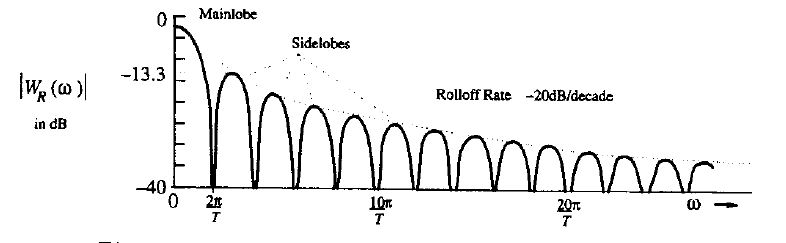
\includegraphics[scale=0.6]{Figures/DFT/amp_spec_rect_window}
\caption{Amplitude Spectrum for Rectangular Window \cite{signal_processing_Lathi}}
\label{fig:DFT:amp_spec_rect_window}
\end{figure}

\end{itemize}

\underline{Example: Effect of Window with a cos Signal}

\begin{itemize}

\item Let $x(t) \, = \, A_1 \, \cos( 2 \pi f_0 \, t \, + \, \phi)$

\item The spectrum of $x(t)$ can be directly obtained using Euler identity

\begin{equation}
    x_c(t) \, = \, \displaystyle\frac{1}{2} \, A_1 \, e^{-j \, \phi} \, e^{-j \,2 \pi f_0 \, t} \, + \, \displaystyle\frac{1}{2} \, A_1 \, e^{j \, \phi} \, e^{j \, 2 \pi f_0 \, t}
\end{equation}


\item The time windowed signal $x_w(t)$:

\begin{equation}
 x_w(t) \, = \, \displaystyle\frac{1}{2} \, A_1 \, e^{-j \, \phi} \, w(t) \, e^{-j \, 2 \pi f_0 \, t} \, + \, \displaystyle\frac{1}{2} \, A_1 \, e^{j \, \phi} \, \, w(t) \, e^{j \, 2 \pi f_0 \, t} 
 \label{Eq:DTF:Window_Eq_1}
\end{equation}

\item Taking the CTFT of \autoref{Eq:DTF:Window_Eq_1} and using the frequency shift property \cite{signal_processing_Lathi} ( $x(t) \, e^{j \, 2 \pi f_0 \, t} \leftrightarrow \, X(F \, - \, f_0)$ ), we have:

\begin{equation}
   X_w(F) \, = \, \displaystyle\frac{1}{2} \, A_1 \, e^{-j \, \phi} \, W(\, F \, + \, f_0 \,)  \, + \, \displaystyle\frac{1}{2} \, A_1 \, e^{j \, \phi} \, \, W(\, F \, - \, f_0 \,)
 \label{Eq:DTF:Window_Eq_2}  
\end{equation}

\item Interpretation of \autoref{Eq:DTF:Window_Eq_2}: the effect of time windowing is to replace each spectral line of the CTFT spectrum with \tbi{scaled copy of}  $W(F)$ centered at the frequency  of the line

\item As an example of a window, we begin with a rectangular one: 

\begin{equation}
\Pi \left(\, \displaystyle\frac{t}{\tau} \,\right) \, \leftrightarrow \, \tau \,  \text{sinc} \left(\, \pi \,F \,  \tau \,  \right)    
\end{equation}


\newpage
\item Visualisation of the computation steps are shown in \autoref{fig:DFT:windowing_modeling_2}

\begin{figure}[h]
\centering
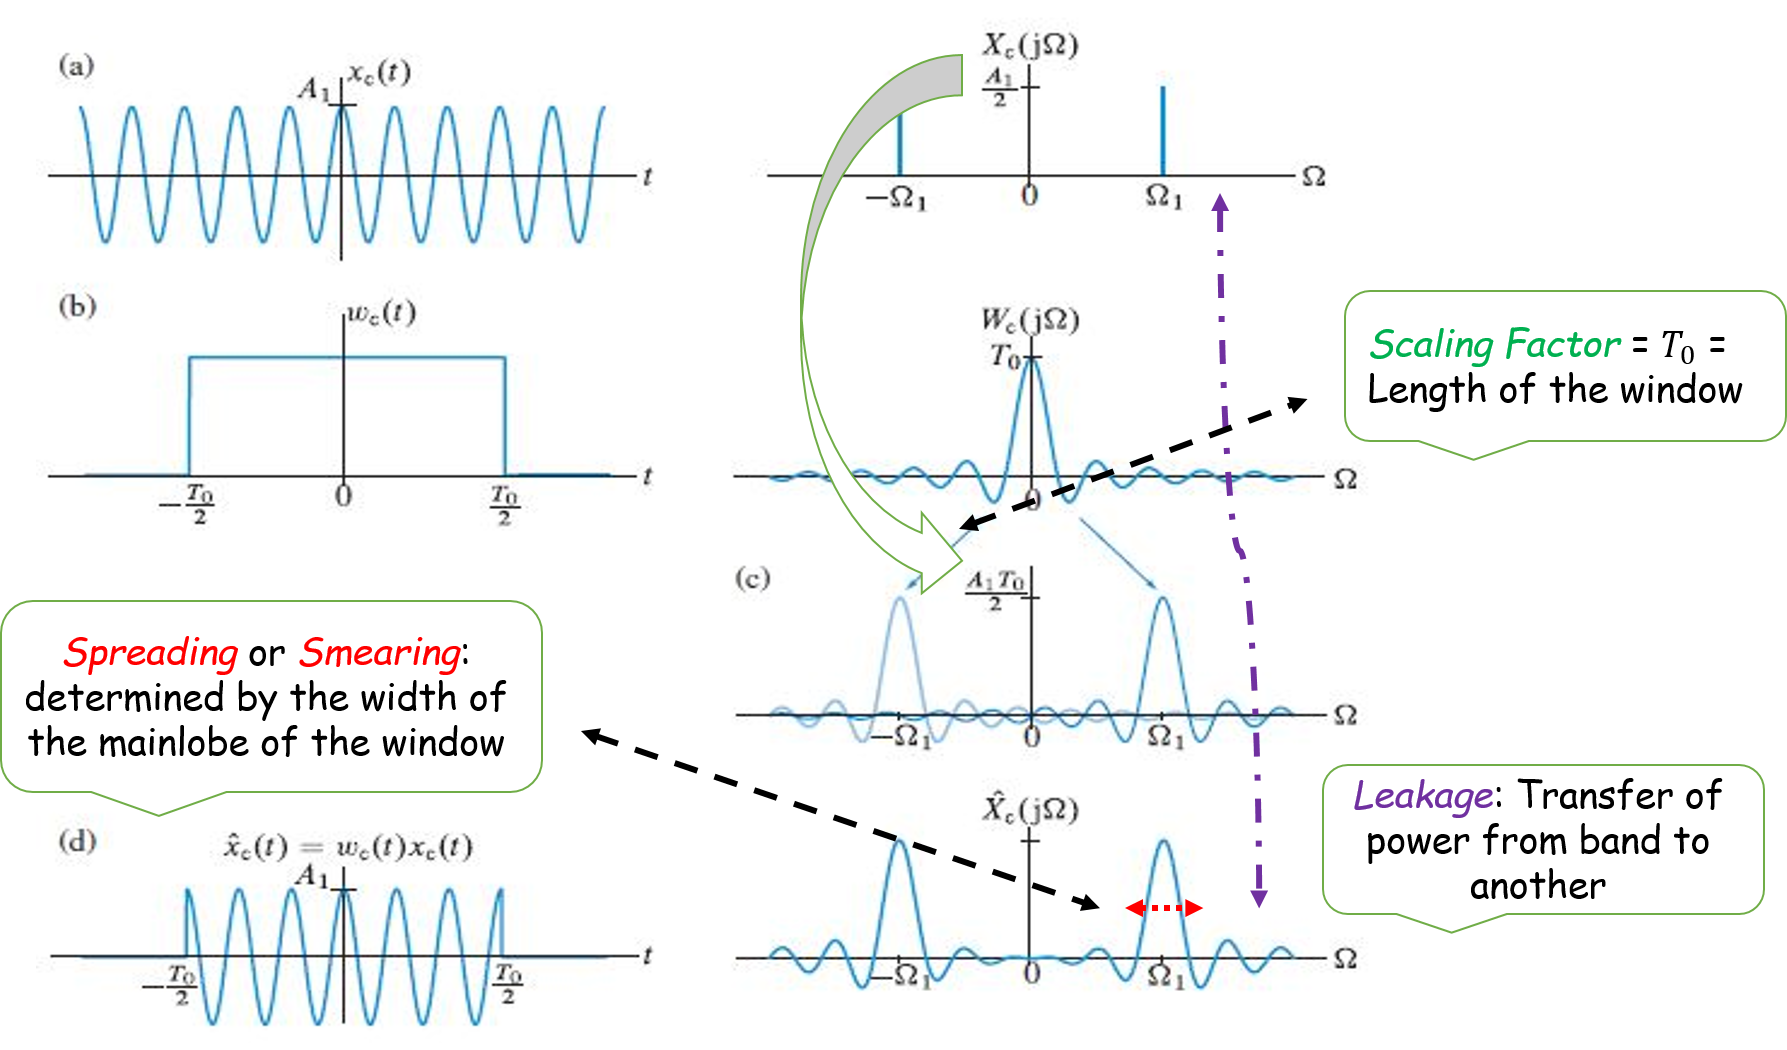
\includegraphics[width = 0.80\textwidth]{Figures/DFT/windowing_modeling_2}
\caption{Windowing Effect on CTFT Amplitude Spectrum}
\label{fig:DFT:windowing_modeling_2}
\end{figure}


3 Things to be noticed from figure \autoref{fig:DFT:windowing_modeling_2} \cite{DSP_DimitrisManolakis}

\begin{enumerate}

\item \tbi{Spectral Spreading} or \tbi{Spectral Smearing}

	\begin{itemize}
	
	\item Controlled by the \tbi{width of the main lobe}	
	
	\item The cosine signal now has spread out after and before $\omega_{c_1}$
	
	\item Smearing can cause \tbi{peak merging }$\leftrightarrow$ reduce the resolvability in the spectrum when have several components close to each other
	
		\begin{itemize}
		\item To be seen in the simulations after
		\end{itemize}
		
	\end{itemize}


\item \tbi{Leakage}:

	\begin{itemize}
	
	\item Controlled by the \tbi{sidelobs} of the rectangular window	
	
	\item Leakage create false peaks due to the power transfer
	
	\item Also it hides any weak frequency components as we will see in the simulation results after
	\end{itemize}


\item Also notice that the amplitude spectrum is multiplied by $T_0$, the length of the window

	\begin{itemize}
	\item This is because the rect window amplitude spectrum has a maximum equal to $T_0$
	\end{itemize}

\end{enumerate}

\end{itemize}

\newpage
\subsection{Simulation Rectangular Window}

First we simulate a DTFT of a rectangular window for different length.

\begin{figure}[h]
\centering
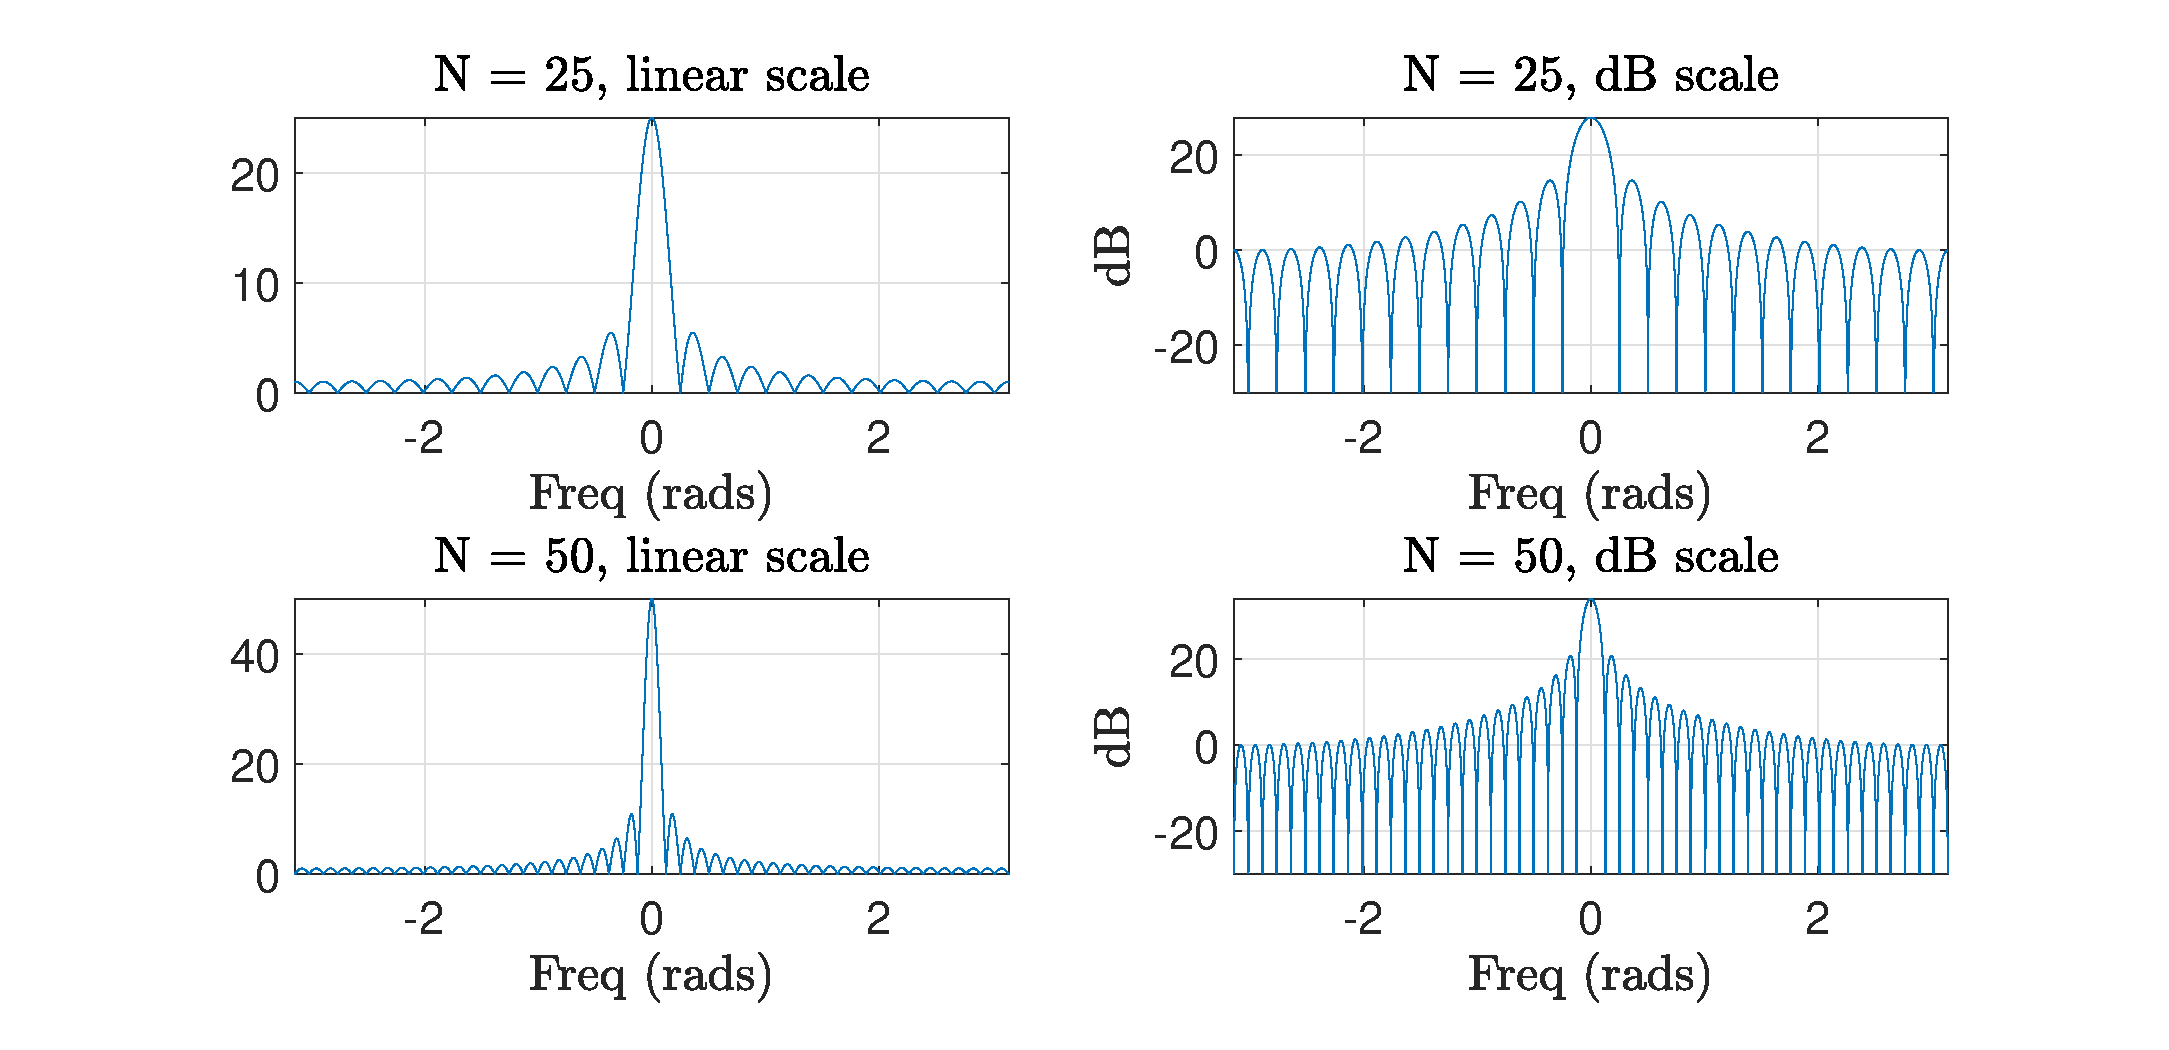
\includegraphics[scale = 0.3]{Figures/Simulation_Sampling_Frequency_Analysis/rect_window_nb_samples}
\caption{DTFT Amplitude Spectrum for the Rectangular Window in Linear and dB Scale}
\label{fig:Simulation_Sampling_Frequency_Analysis:rect_window_nb_samples}
\end{figure}


if we choose \tbi{higher number of samples}

\begin{enumerate}
\item We get a \tbi{narrower main lobe}
	
\item But the \tbi{side lobes doesn't change that much}
\end{enumerate}


\subsection{Simulation 2 Cos Signals}

If the \tbi{cosine signals are too close together}, then doing convolution with our window will add up the 2 cos, and hence we can't distinguish the frequency content of the signals
	
		\begin{itemize}
		\item This is known of \textcolor{red}{peak merging} (loss of spectral resolution) when the 2 spectral line are closer then the width of the main lobe \cite{DSP_DimitrisManolakis}
		\end{itemize}

\begin{figure}[h]
\centering
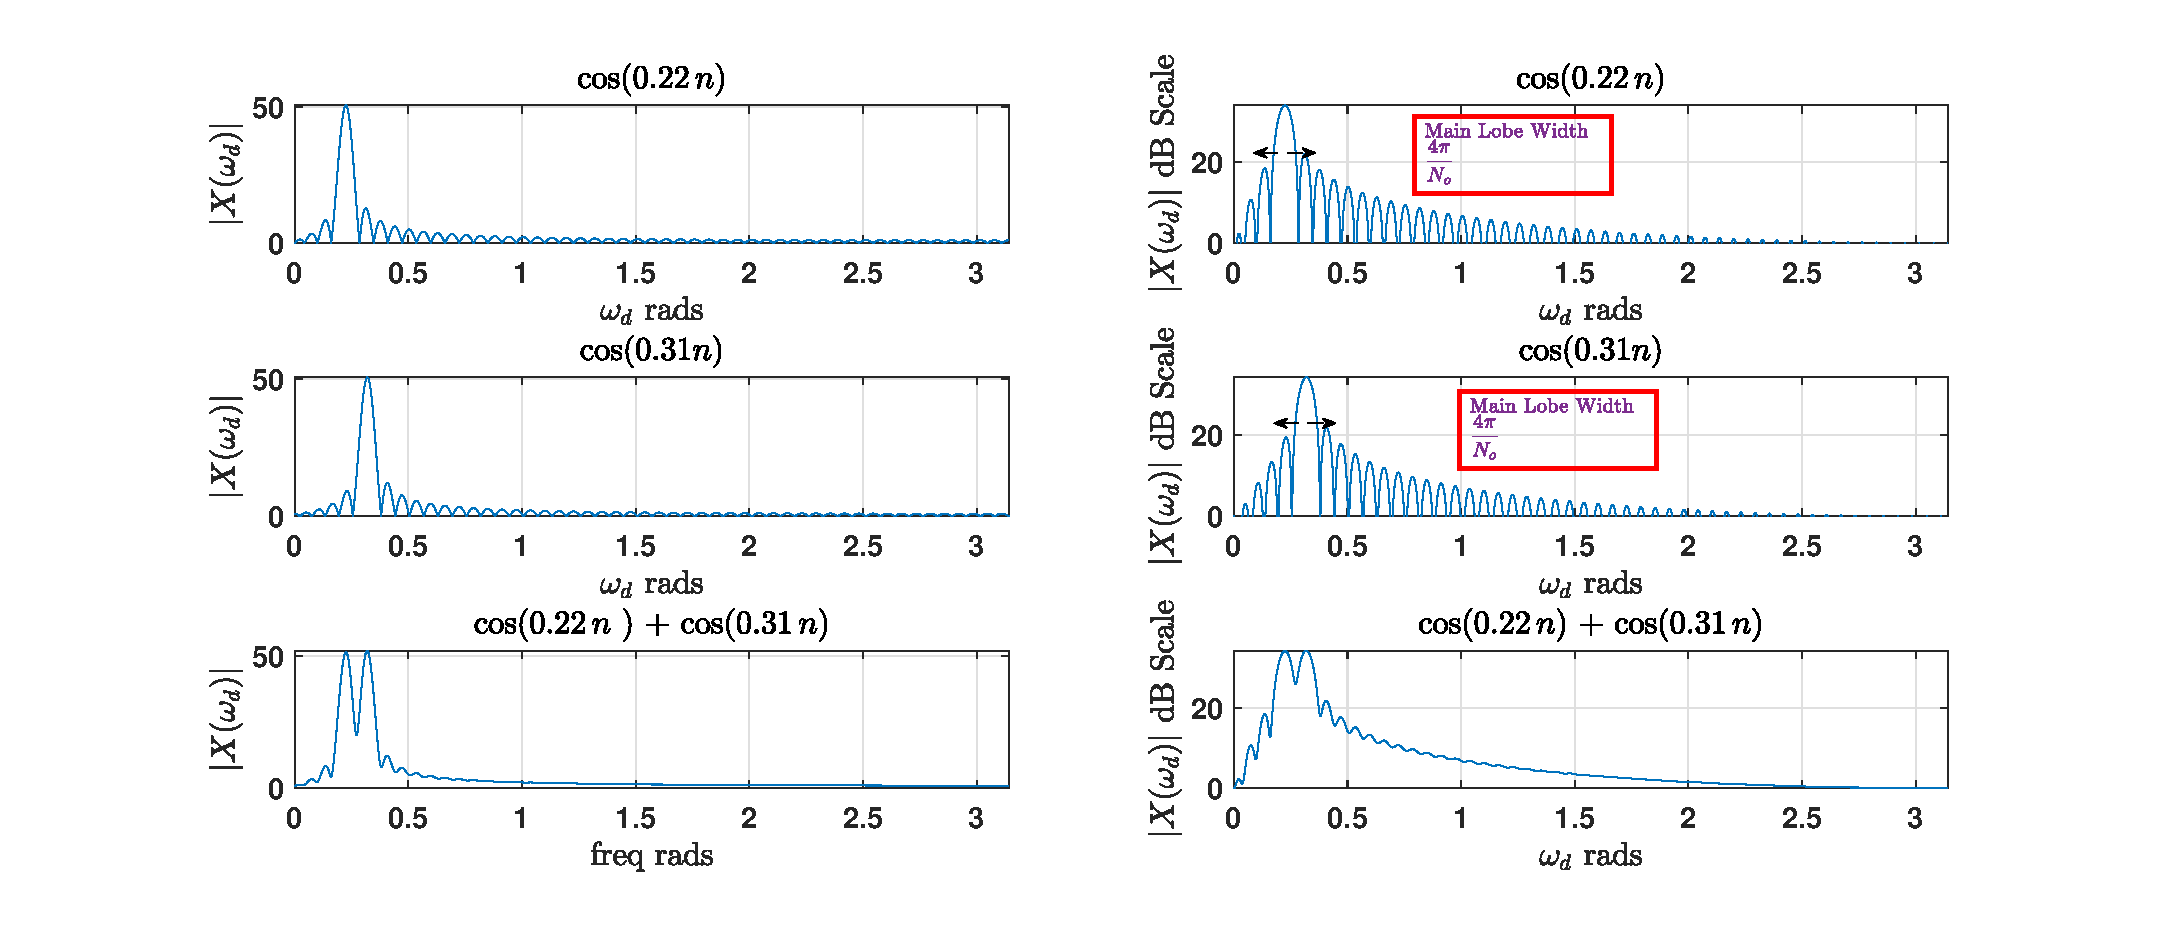
\includegraphics[width = 1\textwidth]{Figures/DFT/spaced_cos}
\caption{Spaced Cos signal}
\label{fig:DFT:spaced_cos}
\end{figure}

\begin{itemize}

\item We have 2 cos signals with discrete frequencies:

	\begin{itemize}
	\item $ \omega_{d_1} \, = \, \displaystyle\frac{7 \pi}{100} \approx \, 0.22$ and $ \omega_{d_2} \, = \, \displaystyle\frac{10 \pi}{100} \approx \, 0.31$ 
	
	
	\end{itemize}

\item Width of the main lobe $ = \displaystyle\frac{4 \pi}{N} \, = \, \displaystyle\frac{4 \pi}{100}$

	\begin{itemize}
	\item Where $N$ is the length of the rectangular window
	\end{itemize}

\item Spectral separation between signals $= \displaystyle\frac{10 \pi}{100} \, - \, \displaystyle\frac{7 \pi}{100} \, = \, \displaystyle\frac{3 \pi}{100}$

\item Separation rule: Width of the main lobe $\leq$ Spectral separation between signals $\leftrightarrow \,\displaystyle\frac{4 \pi}{100} \,\leq \,  \displaystyle\frac{3 \pi}{100} \, \leftrightarrow$ rule is almost verified with some errors however

	\begin{itemize}
	\item  But still we are able to distinguish the 2 components
	\end{itemize}
	
\end{itemize}

\underline{1 Weak and 1 Strong Signal}\\

Trickiest part: don't forget \tbi{the side lobes}

\begin{itemize}
	
\item Case of 1 strong and the $\mathrm{2}^\mathrm{nd}$ is weak
	
\item Even if the $\mathrm{2}^\mathrm{nd}$ component is far from the $\mathrm{1}^\mathrm{st}$ one, the $\mathrm{2}^\mathrm{nd}$ could be a small one and add up with the side lobes of the $\mathrm{1}^\mathrm{st}$ one (the strong one)

\end{itemize}


\begin{figure}[h]
\centering
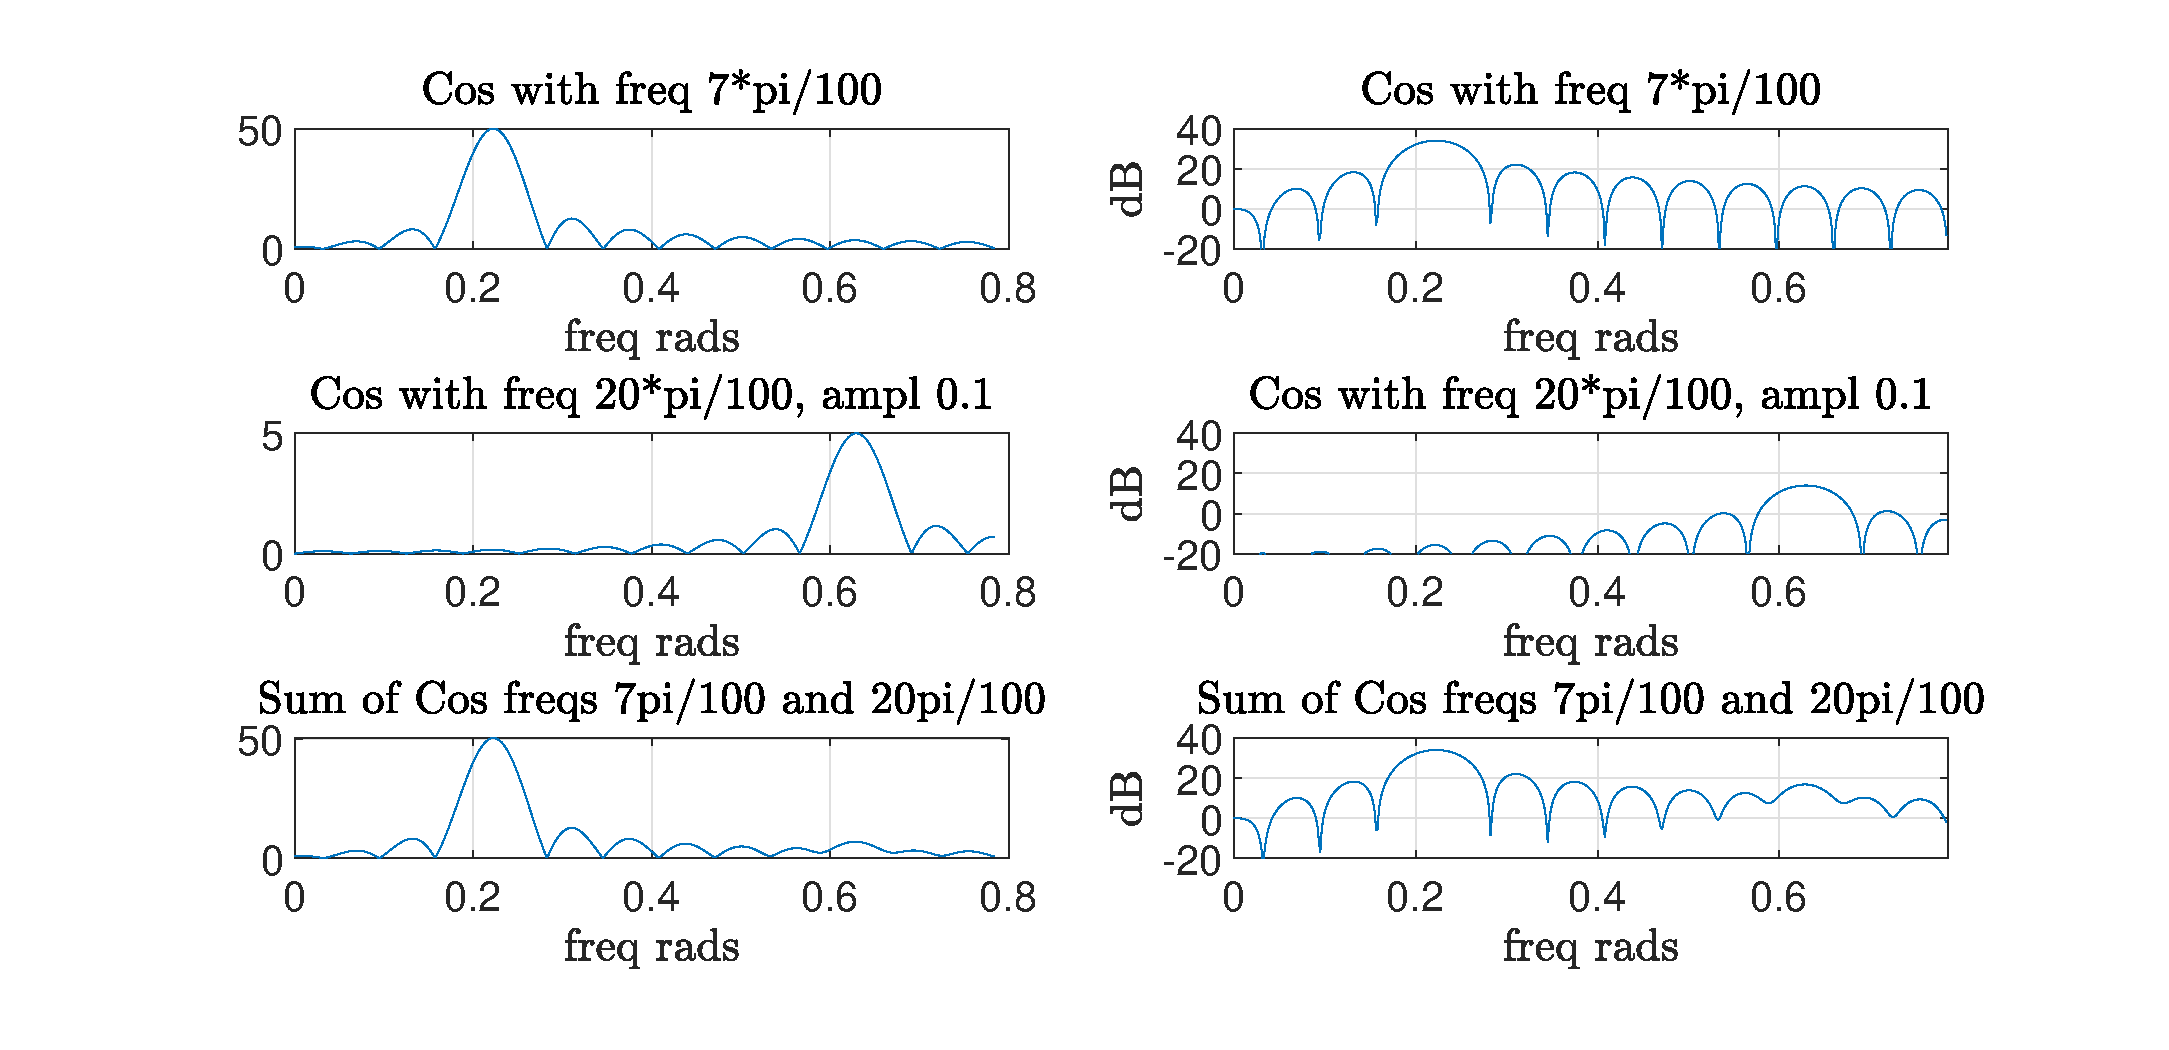
\includegraphics[width = 1\textwidth]{Figures/Simulation_Sampling_Frequency_Analysis/spaced_weak_cos}
\caption{Well separated signals but with weak components}
\label{fig:Simulation_Sampling_Frequency_Analysis:closed_cos}
\end{figure}

\subsection{Window Choice}

\begin{itemize}

\item In previous part, we have seen the effect of side lobs in a rectangular window:

	\begin{enumerate}
	\item Very high resolution $\leftrightarrow$ narrow main lobe
	
	\item Not very efficient dynamic range $\leftrightarrow$ side lobe effects still high even if we truncate less
	\end{enumerate}


\item In rectangular window, we have a sudden transition from $1 \rightarrow 0$ or $0 \rightarrow 1$ in the time domain, which make the side lobes to be appear in the frequency domain (in CTFT or DTFT Spectrum)

\item This was the motivation for designing other choices of windows: \tbi{trade-off between resolution and dynamic range}

\item Design criteria for \tbi{good window}: 

	\begin{enumerate}
	\item Narrow mainlobe
	
	\item Weak side lobes
	\end{enumerate}


\item Different Window Types

\begin{figure}[h]
\centering
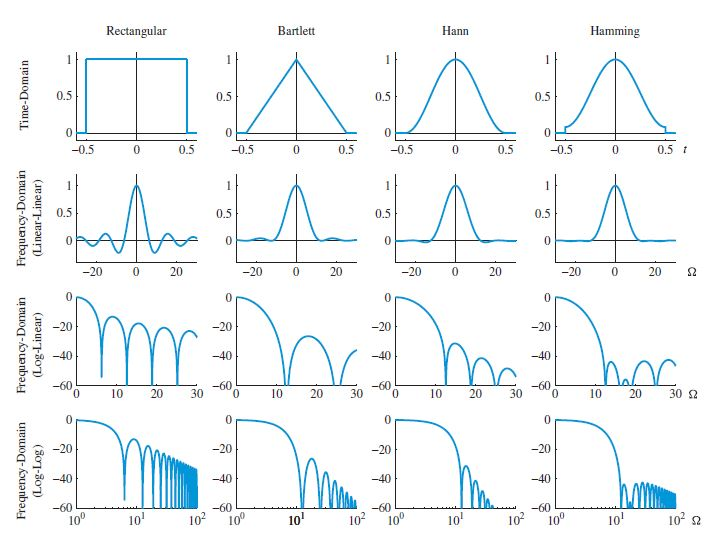
\includegraphics[scale=0.4]{Figures/DFT/other_windows}
\caption{Time-domain and frequency-domain characteristics of continuous-time rectangular, Bartlett (triangular), Hann, and Hamming windows \cite{DSP_DimitrisManolakis}}
\label{fig:DFT:other_windows}
\end{figure}


\begin{figure}[h]
\centering
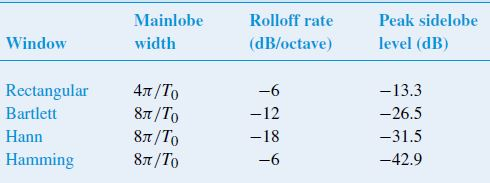
\includegraphics[scale=0.6]{Figures/DFT/other_windows_2}
\caption{Some continuous-time windows and their characteristics \cite{DSP_DimitrisManolakis}}
\label{fig:DFT:other_windows}
\end{figure}

\item Rectangular window has the narrower main lobe $\leftrightarrow$ highest resolution

	\begin{itemize}
	\item However, their side lobes are relatively high $\leftrightarrow$ poorest dynamic range
	\end{itemize}

\item Hamming window has a smoother transition in the time domain from $1 \rightarrow 0$

	\begin{itemize}
	\item Hence it has a wider mainlobe compared to the rectangular window $\leftrightarrow$ lower resolution
	
	\item But lower side lobes $\leftrightarrow$ higher dynamic range
	\end{itemize}

\item Chebyscheve window: we can control the side lobes height, and it has equal height side lobes

	\begin{itemize}
	\item The weaker the side lobes the more the transition is smooth
	
	\item Chebychev with -30 dB attenuation: narrower main lobe but high side lobes
	
	\item Chebychev with -70 db has quite the opposite compared to the -30 dB attenuation
	\end{itemize}

\item As a general rule: the more we push down the side lobes in the frequency domain (hence better dynamic range) $\leftrightarrow$ the main lobe will get higher (lower resolution)


\end{itemize}

\subsection{DTFT Spectrum Using Different Window Type}

\begin{itemize}

\item Example: $x[k] \, = \,\displaystyle\sum_{i \, = \, 1}^{i \, = \, 3} \text{Components}_i$

\begin{itemize}
\item $\text{Component 1 } = \, \text{cos} \left(\, \displaystyle\frac{\pi}{10} \, k \,\right) $
\item $ \text{Component 2 } = \,  \text{cos} \left(\, \displaystyle\frac{\pi}{8} \, k \, + \, \displaystyle\frac{\pi}{3} \right) $
\item $ \text{Component 3 } =  0.01 \, \text{cos} \left(\, \displaystyle\frac{4 \pi}{10} \, k \, - \,\displaystyle\frac{3 \pi }{5} \right) $ 
\end{itemize}


\item 2 criteria to be tested via the discrete signal $x[k]$: Resolution and Dynamic Range

 \begin{itemize}
 \item Resolution: the sum of 2 close signal $\leftrightarrow$ controlled by the width the main lobe
 
 \item Dynamic Range: displaying weak component $\leftrightarrow$ controlled by the height of the side lobes
 \end{itemize}

\newpage
\begin{figure}[h]
\centering
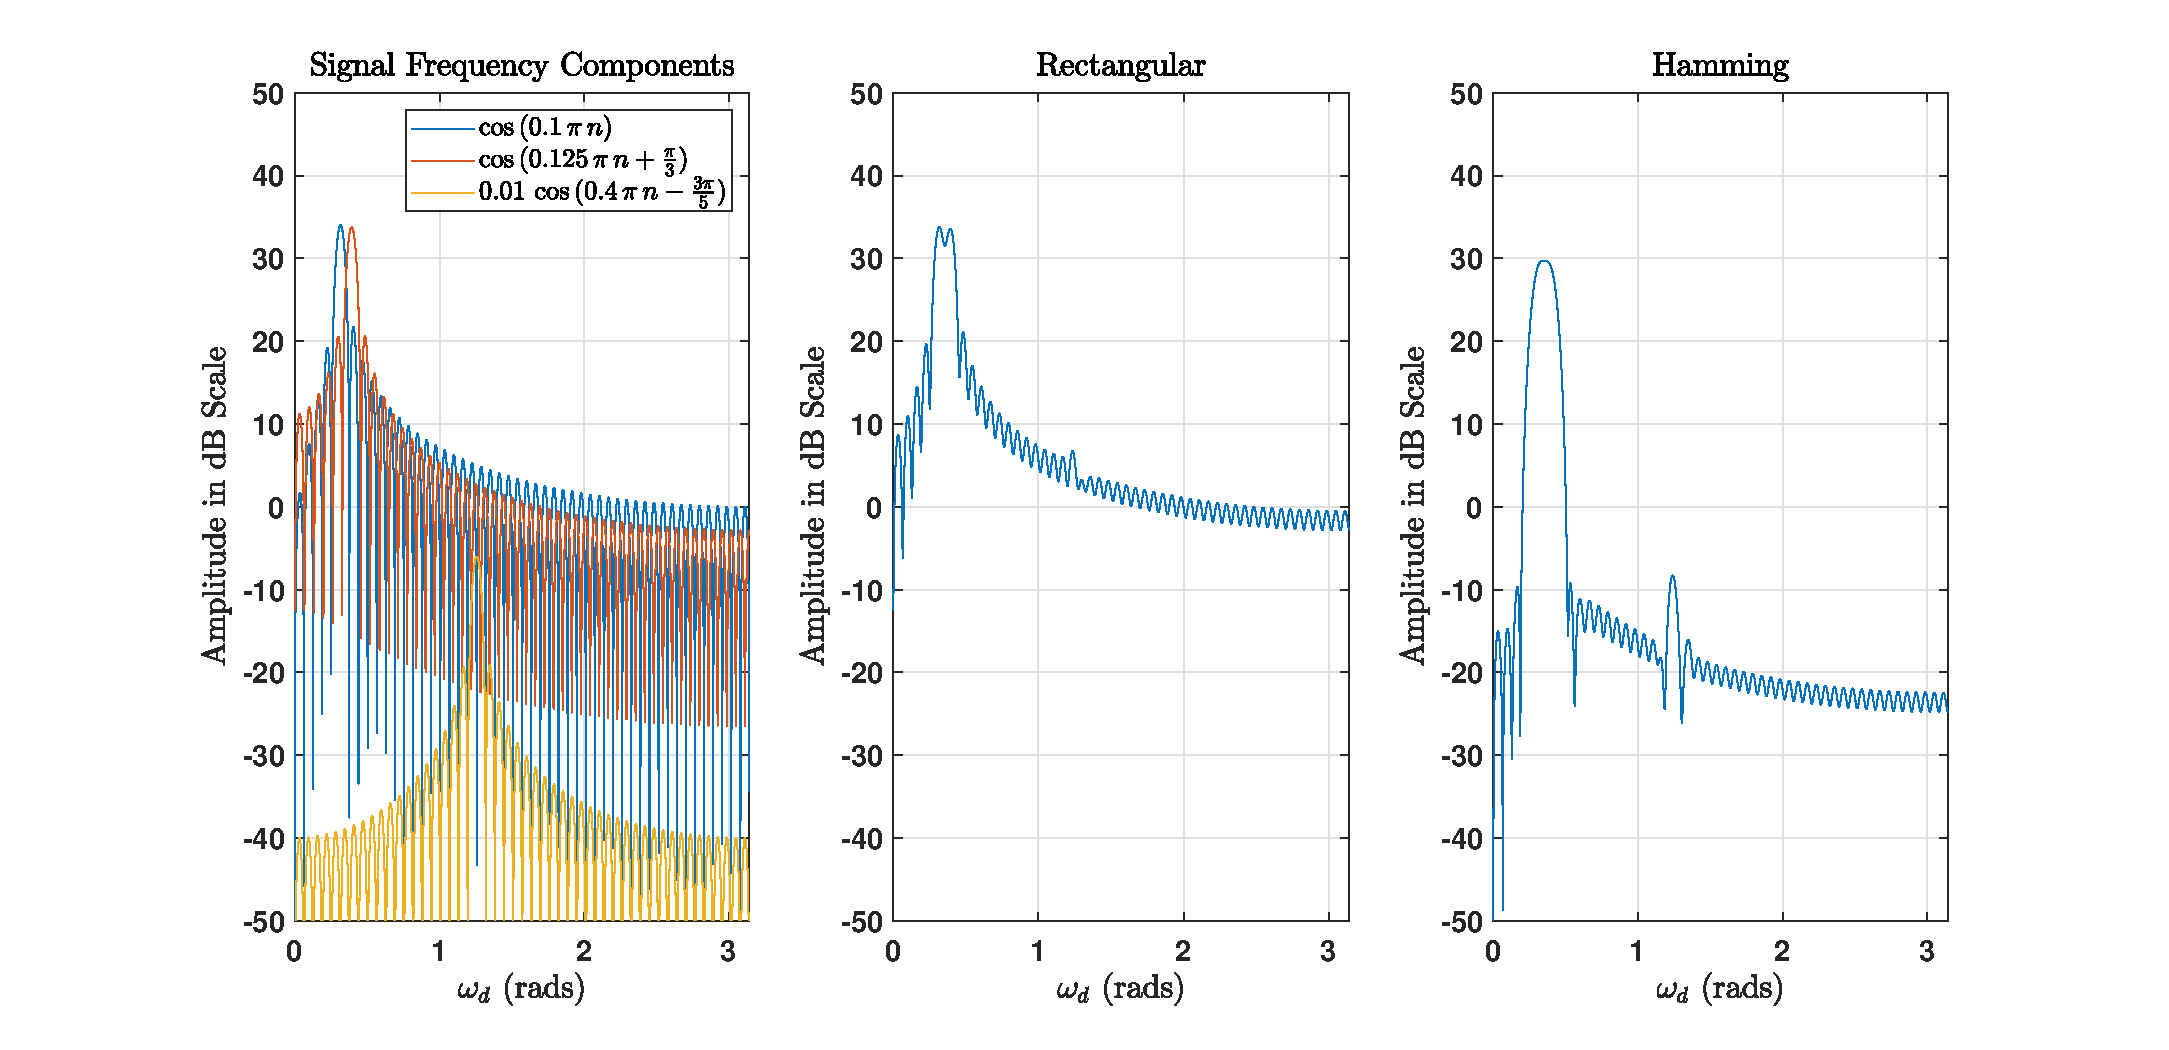
\includegraphics[scale=0.5]{Figures/DFT/sum_of_cos_rect_and_hamm.eps}
\caption{Rectangular and Hamming Window}
\label{fig:Papers:aliasing}
\end{figure}


\item In rectangular window:

	\begin{itemize}
	\item the 2 components  can be distinguished
	
	\item However the $\mathrm{3}^\mathrm{rd}$ components having a small amplitude has disappeared in the side lobes

	\begin{itemize}
	\item It barely  we can see it
	
	\item If we have some noisy data, it will completely		 gone
	\end{itemize}		

	\end{itemize}
	
\item In Hamming window:

\begin{itemize}
\item The 2 cos peaks has merged 

\item But the weak components is detected better then the rectangular window
\end{itemize}

\newpage

\begin{figure}[h]
\centering
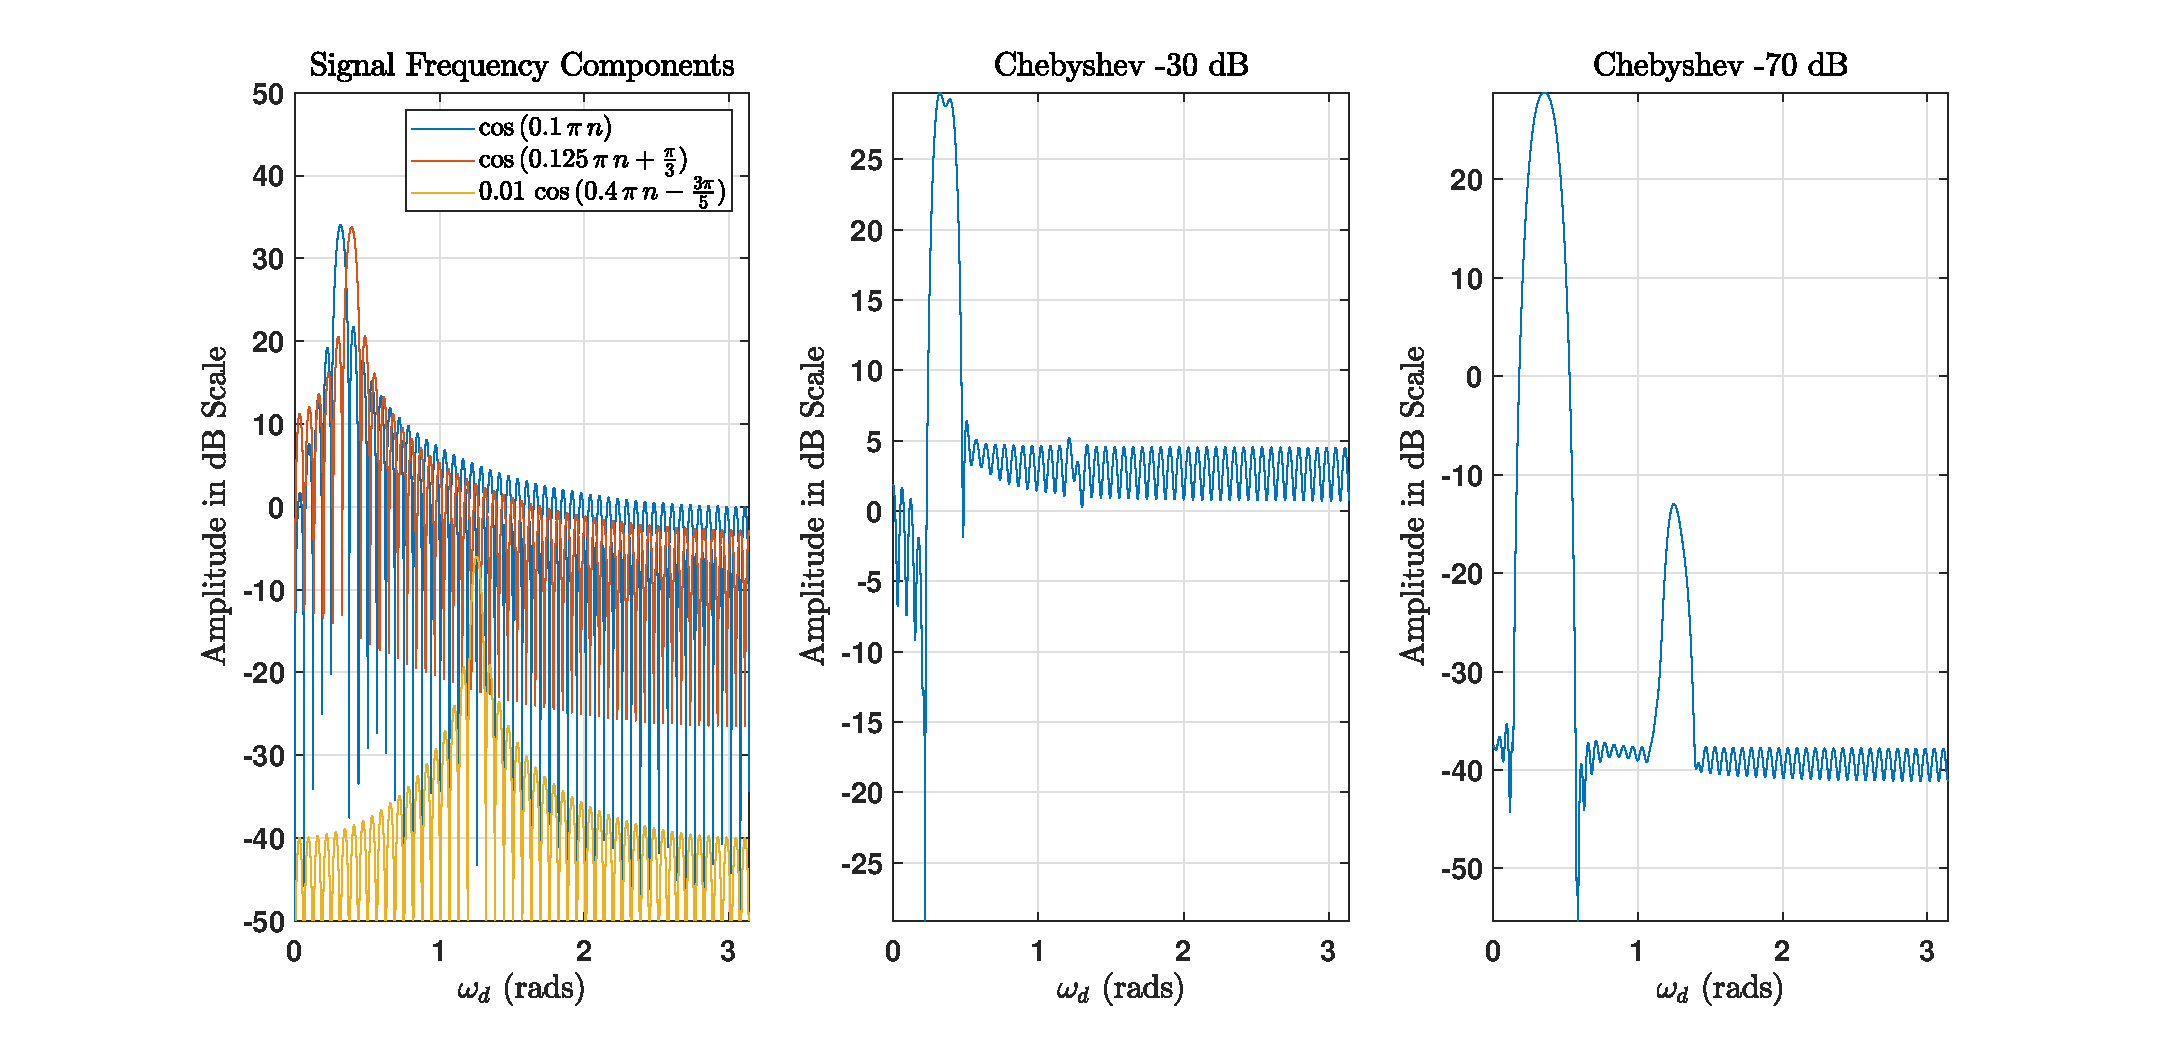
\includegraphics[scale=0.5]{Figures/DFT/sum_of_cos_chebyshev.eps}
\caption{Chebychves Window with -30 dB and -70 dB side lobes attenuation}
\label{fig:DFT:sum_of_cos_chebyshev}
\end{figure}

\item In -30 dB case:

	\begin{itemize}
	\item We can (although it is difficult) to see that we have 2 frequency components $\leftrightarrow$ good resolution
	
	\item However the weak component have vanished $\leftrightarrow$ poorer dynamic range
	\end{itemize}

\item In -70 dB case we have opposite results

	\begin{itemize}
	\item Since thee side lobes now are more attenuated, we can detect the weak component
	
	\item Of course in the price of poorer resolution as we can see, the 2 components are gone now
	\end{itemize}

\end{itemize}


\subsection{CTFT Analysis Using Different Window}

\begin{itemize}

\item We try to see now the effect of windows on CTFT spectrum for a damped cos signals given by:

\begin{equation*}
\begin{array}{rcl}
x(t) \, &=& \, e^{-0.1 \,t} \, \left[\, \text{cos}\left( \, 10 \, t \, \right) \, + \, \text{cos}\left( \, 12 \, t \, \right)  \,\right] \, u(t) \\ \\
X(\omega_c) \, &=& \, \displaystyle\frac{\, 0.1 \, + \, j \, \omega_c}{ \left( \, 0.1 \, + \, j \, \omega_c  \,  \right)^2    \, + \, 10^2} \, + \, \displaystyle\frac{0.1 \,+ \, j \, \omega_c}{ \left( \, 0.1 \, + \, j \, \omega_c  \,  \right)^2    \, + \, 12^2}
\end{array}
\end{equation*}


\begin{figure}[h]
\centering
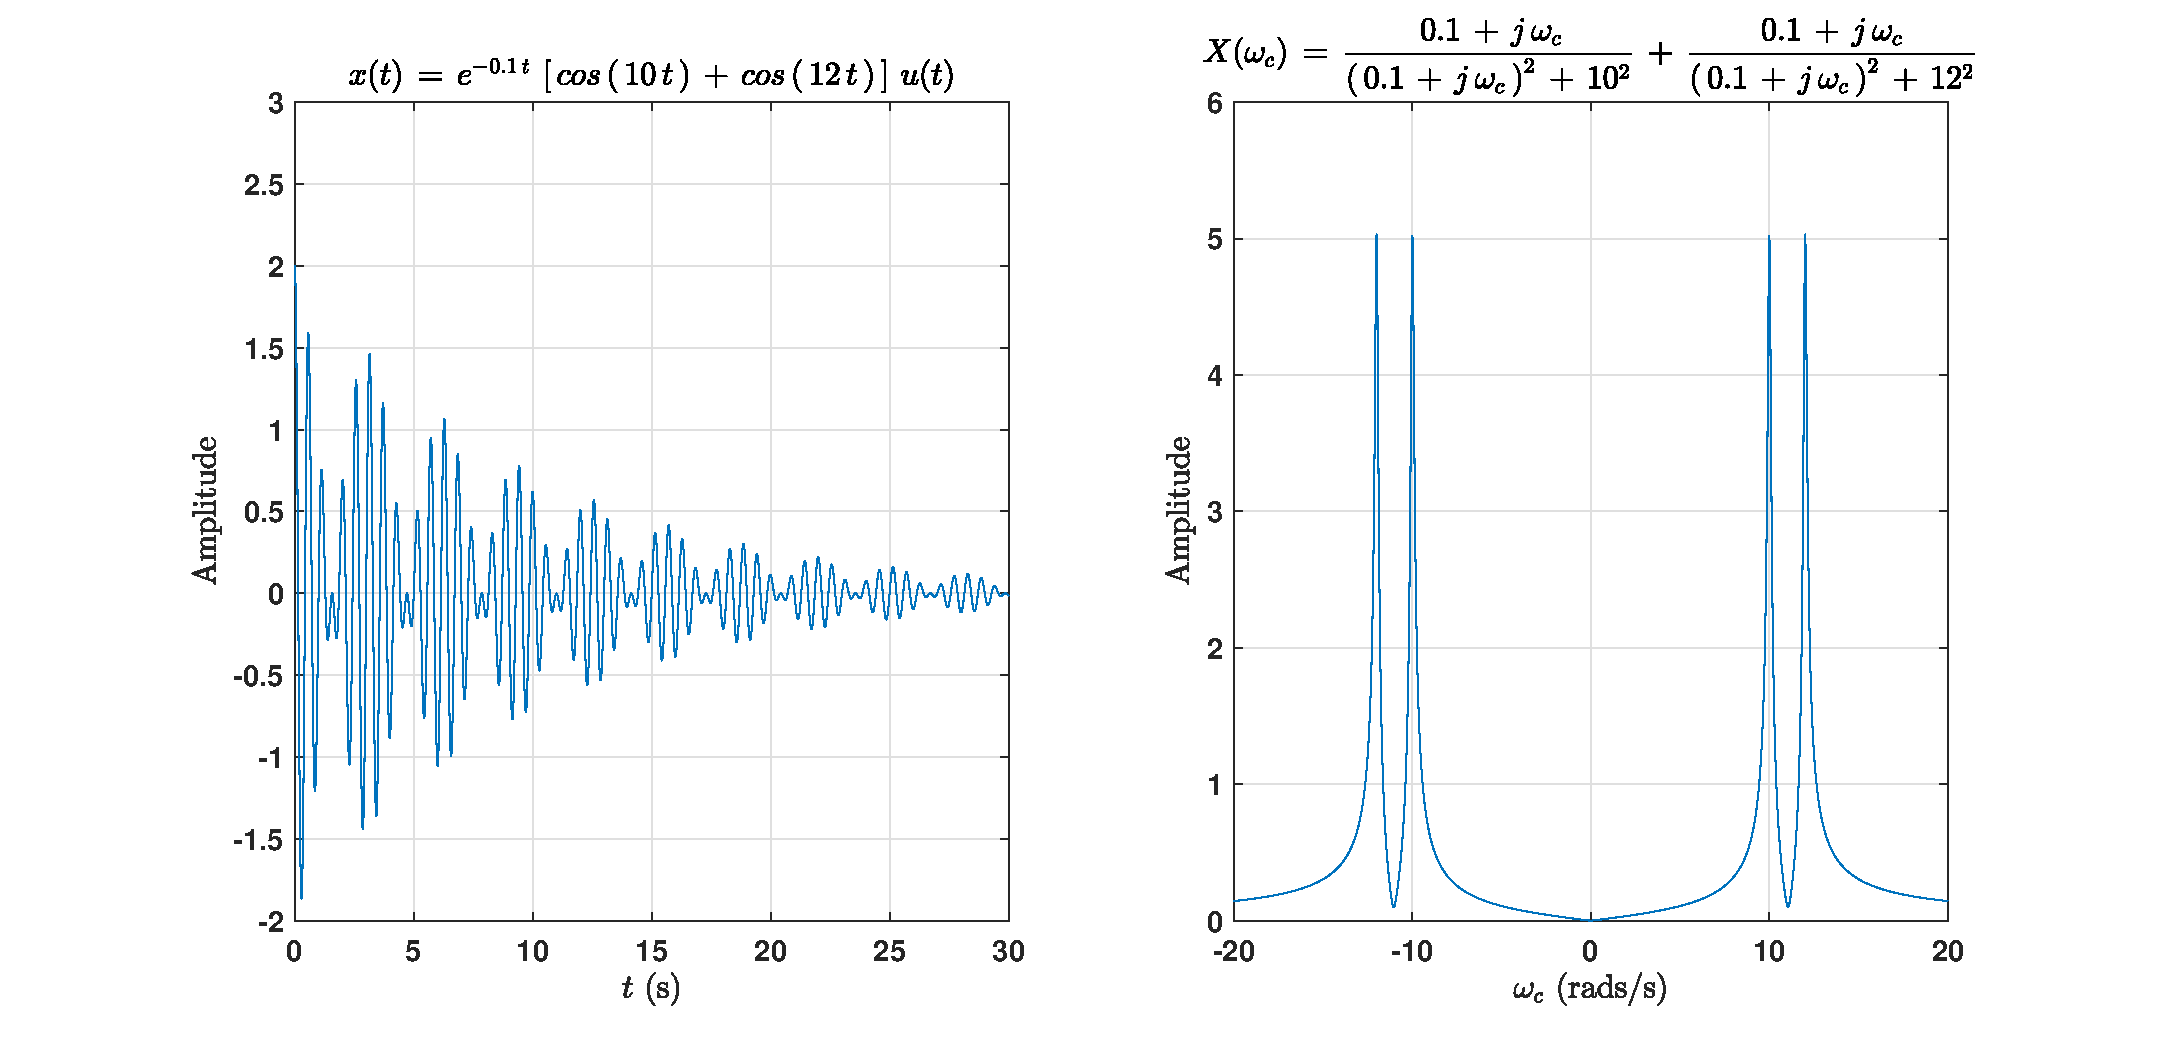
\includegraphics[scale=0.30]{Figures/DFT/damped_cosines_and_spectrum.eps}
\caption{$x(t)$ along with its Amplitude Spectrum}
\label{fig:DFT:damped_cosines_and_spectrum}
\end{figure}

\item $X(\omega_c)$ is not a bandlimited signal, so we need to choose a maximum frequency

	\begin{itemize}
	\item Since we can visualize that after 12 rad/s the spectrum roll off, we choose effective bandwidth of $B \, = \, 300$ rad/s $\rightarrow \, T_s \, = \, 0.01$ s
	\end{itemize}



\item We have 2 damped frequency components at 10 and 12 rad/s. Spectral Separation between these 2 components is $12 \, - \, 10 \,  = \, 2 $ rad/s 

\item Recall that the width of the main lobe need to be smaller than the spectral separation

\item We choose to see details at 2 resolution using rectangular window:

	\begin{enumerate}
	\item $\displaystyle\frac{2 \pi}{5} \, \approx \, 1.2566 <<  2$ rad/s
	
		\begin{itemize}
		\item $\displaystyle\frac{4 \pi}{\text{Signal Duration}} \, = \,   \displaystyle\frac{4 \pi}{T_s \, N} \leq \, \displaystyle\frac{2 \pi}{5} \rightarrow \, N \, \geq \, 1000 $ samples
		\end{itemize}
		
	\item We increase resolution times 5: $\displaystyle\frac{2 \pi}{25} \, \approx \, 0.2513$
	
	\begin{itemize}
		\item $\displaystyle\frac{4 \pi}{\text{Signal Duration}} \, = \,   \displaystyle\frac{4 \pi}{T_s \, N} \leq \, \displaystyle\frac{2 \pi}{25} \rightarrow \, N \, \geq \, 5000 $ samples
		\end{itemize}

	\end{enumerate}
	
\begin{figure}[h]
\centering
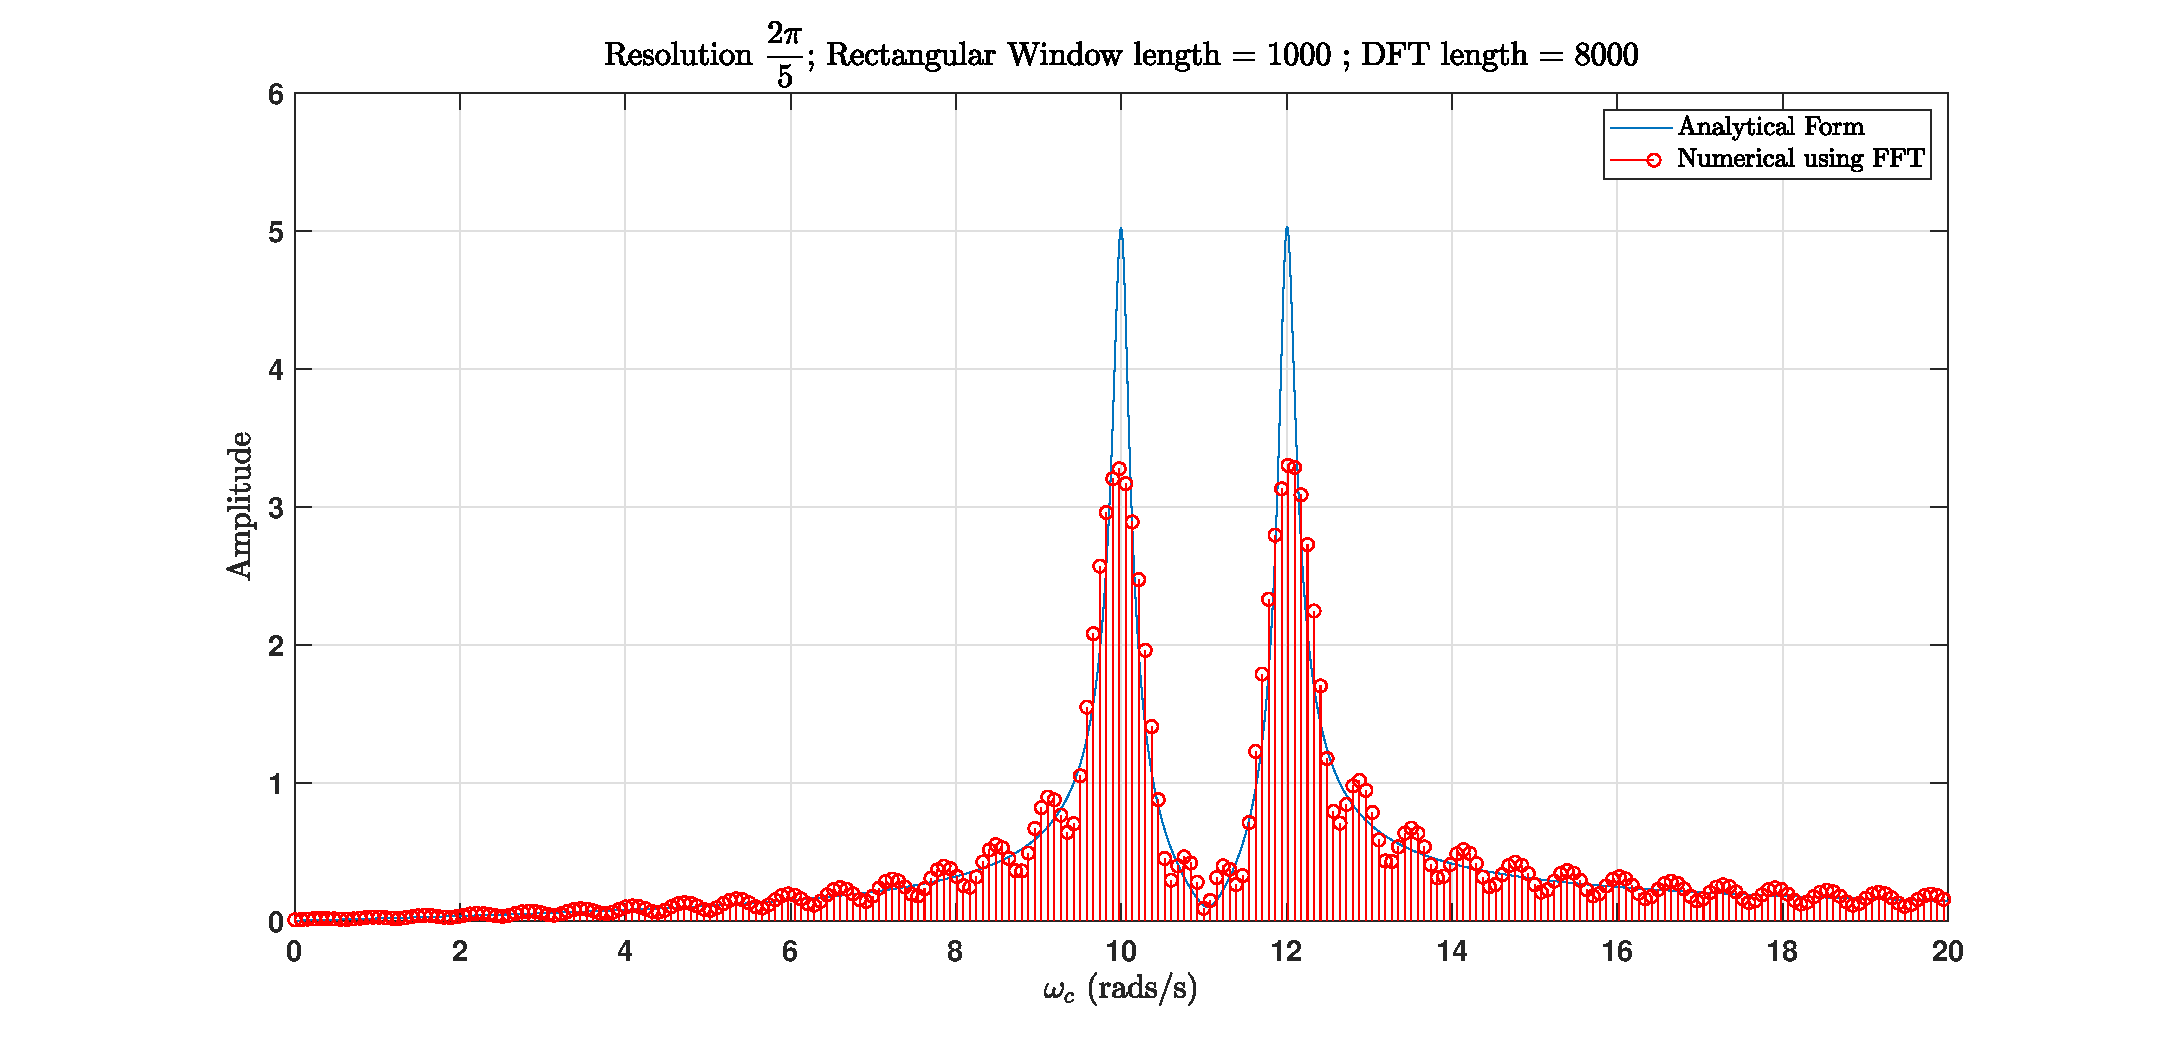
\includegraphics[scale=0.30]{Figures/DFT/spectrum_rect_window_length_1000.eps}
\label{fig:DFT:spectrum_rect_window_length_1000}
\end{figure}

\begin{itemize}

\item DFT Values are distorted

\item Some ripples at the tails

\end{itemize}


\item Increasing resolution 5 times from $\displaystyle\frac{2 \pi}{5} \rightarrow \displaystyle\frac{2 \pi}{25}$ (narrower main lobe)


	\begin{itemize}
	\item Better DFT Values and  No ripples at the tails
	\end{itemize}


\begin{figure}[h]
\centering
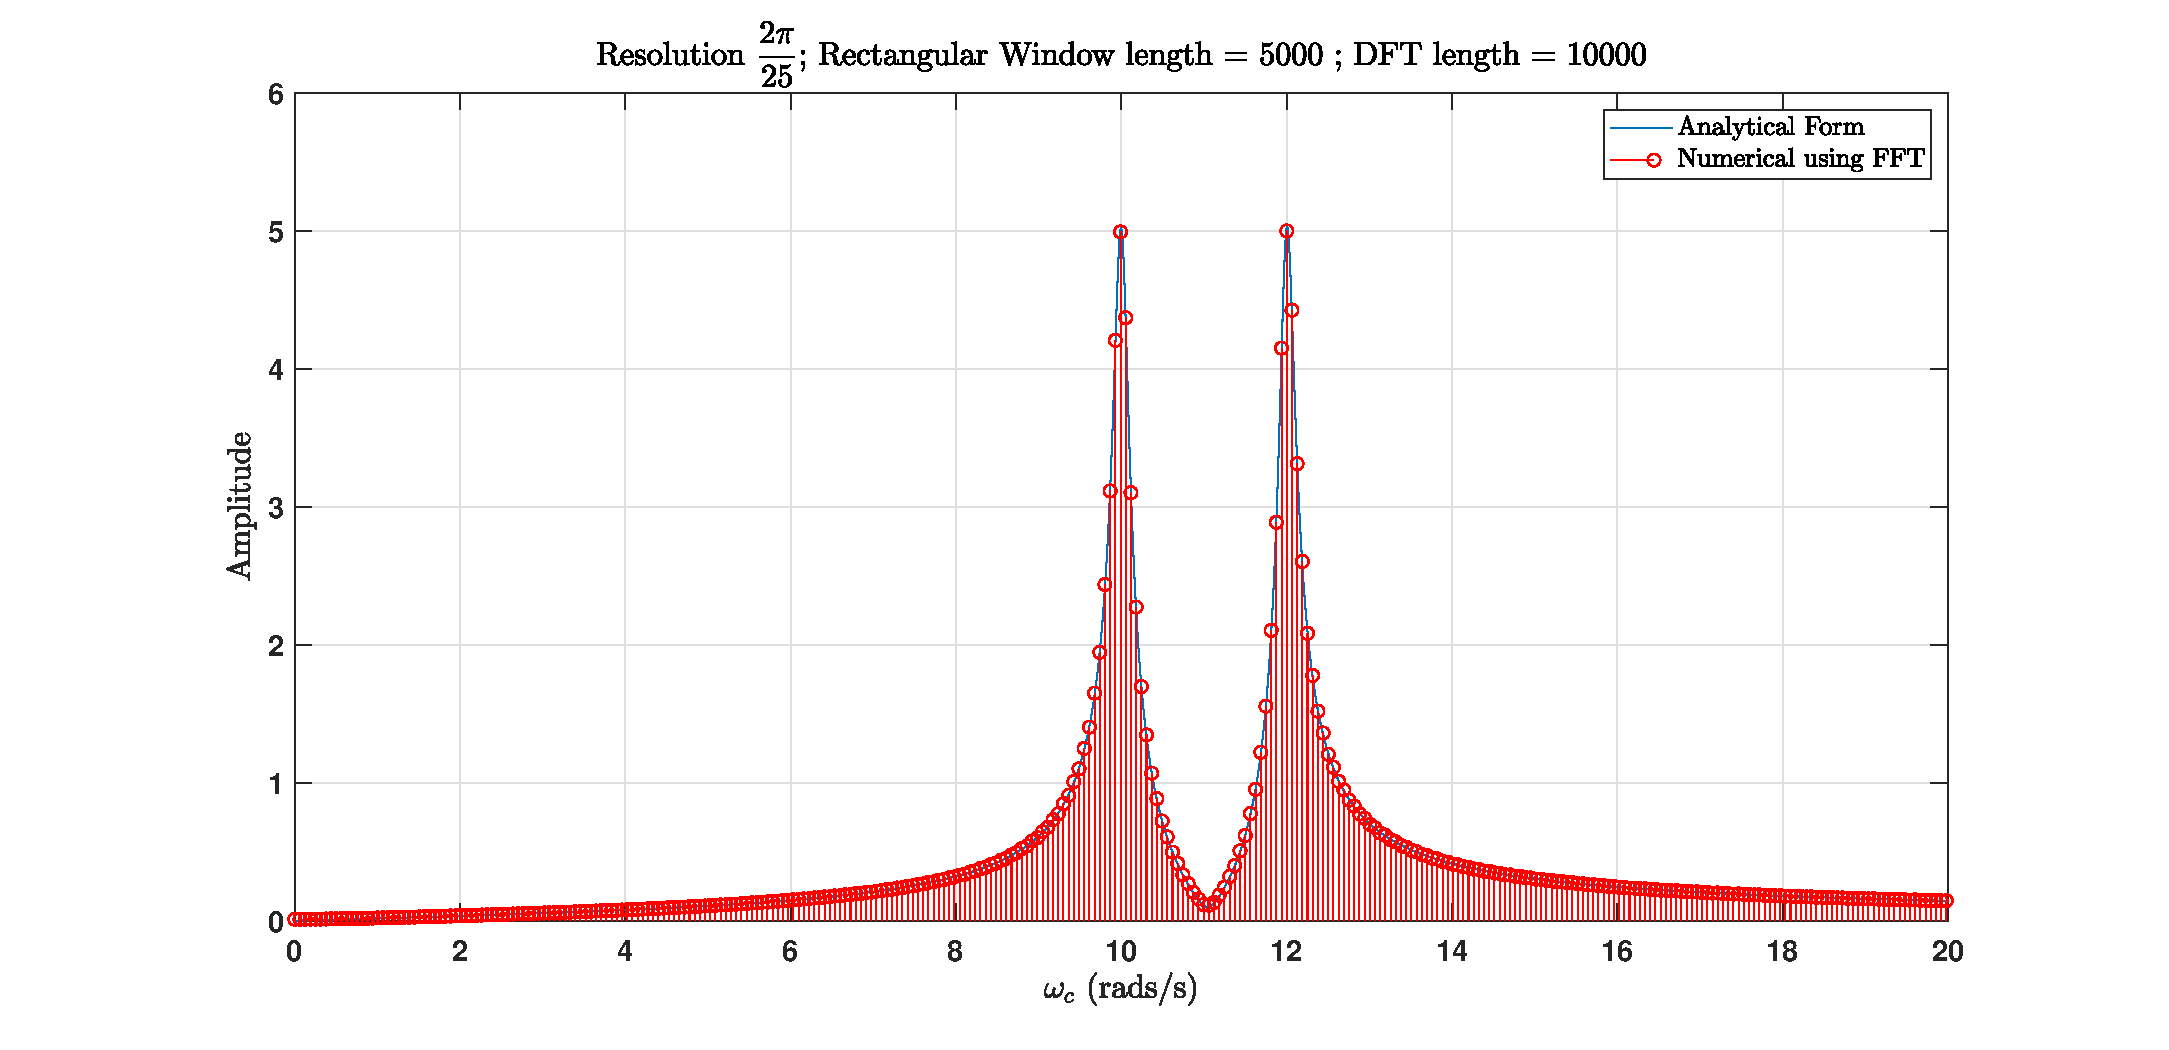
\includegraphics[scale=0.26]{Figures/DFT/spectrum_rect_window_length_5000.eps}
\label{fig:DFT:spectrum_rect_window_length_1000}
\end{figure}

\item Trying Different type of Windows: Hamming window for example, with the best observed resolution which is $  \displaystyle\frac{2 \pi}{25}$

\item Hamming Length:

	\begin{itemize}
	\item $\displaystyle\frac{8 \pi}{\text{Signal Duration}} \, = \,   \displaystyle\frac{8 \pi}{T_s \, N} \leq \, \displaystyle\frac{2 \pi}{5} \rightarrow \, N \, \geq \, 10^4 $ samples
	
	\item Rectangular window length was 5000 samples for a resolution  of $  \displaystyle\frac{2 \pi}{25}$
	
	\item Hamming need 2 times more samples then rectangular to observe same level of details
	\end{itemize}


\begin{figure}[h]
\centering
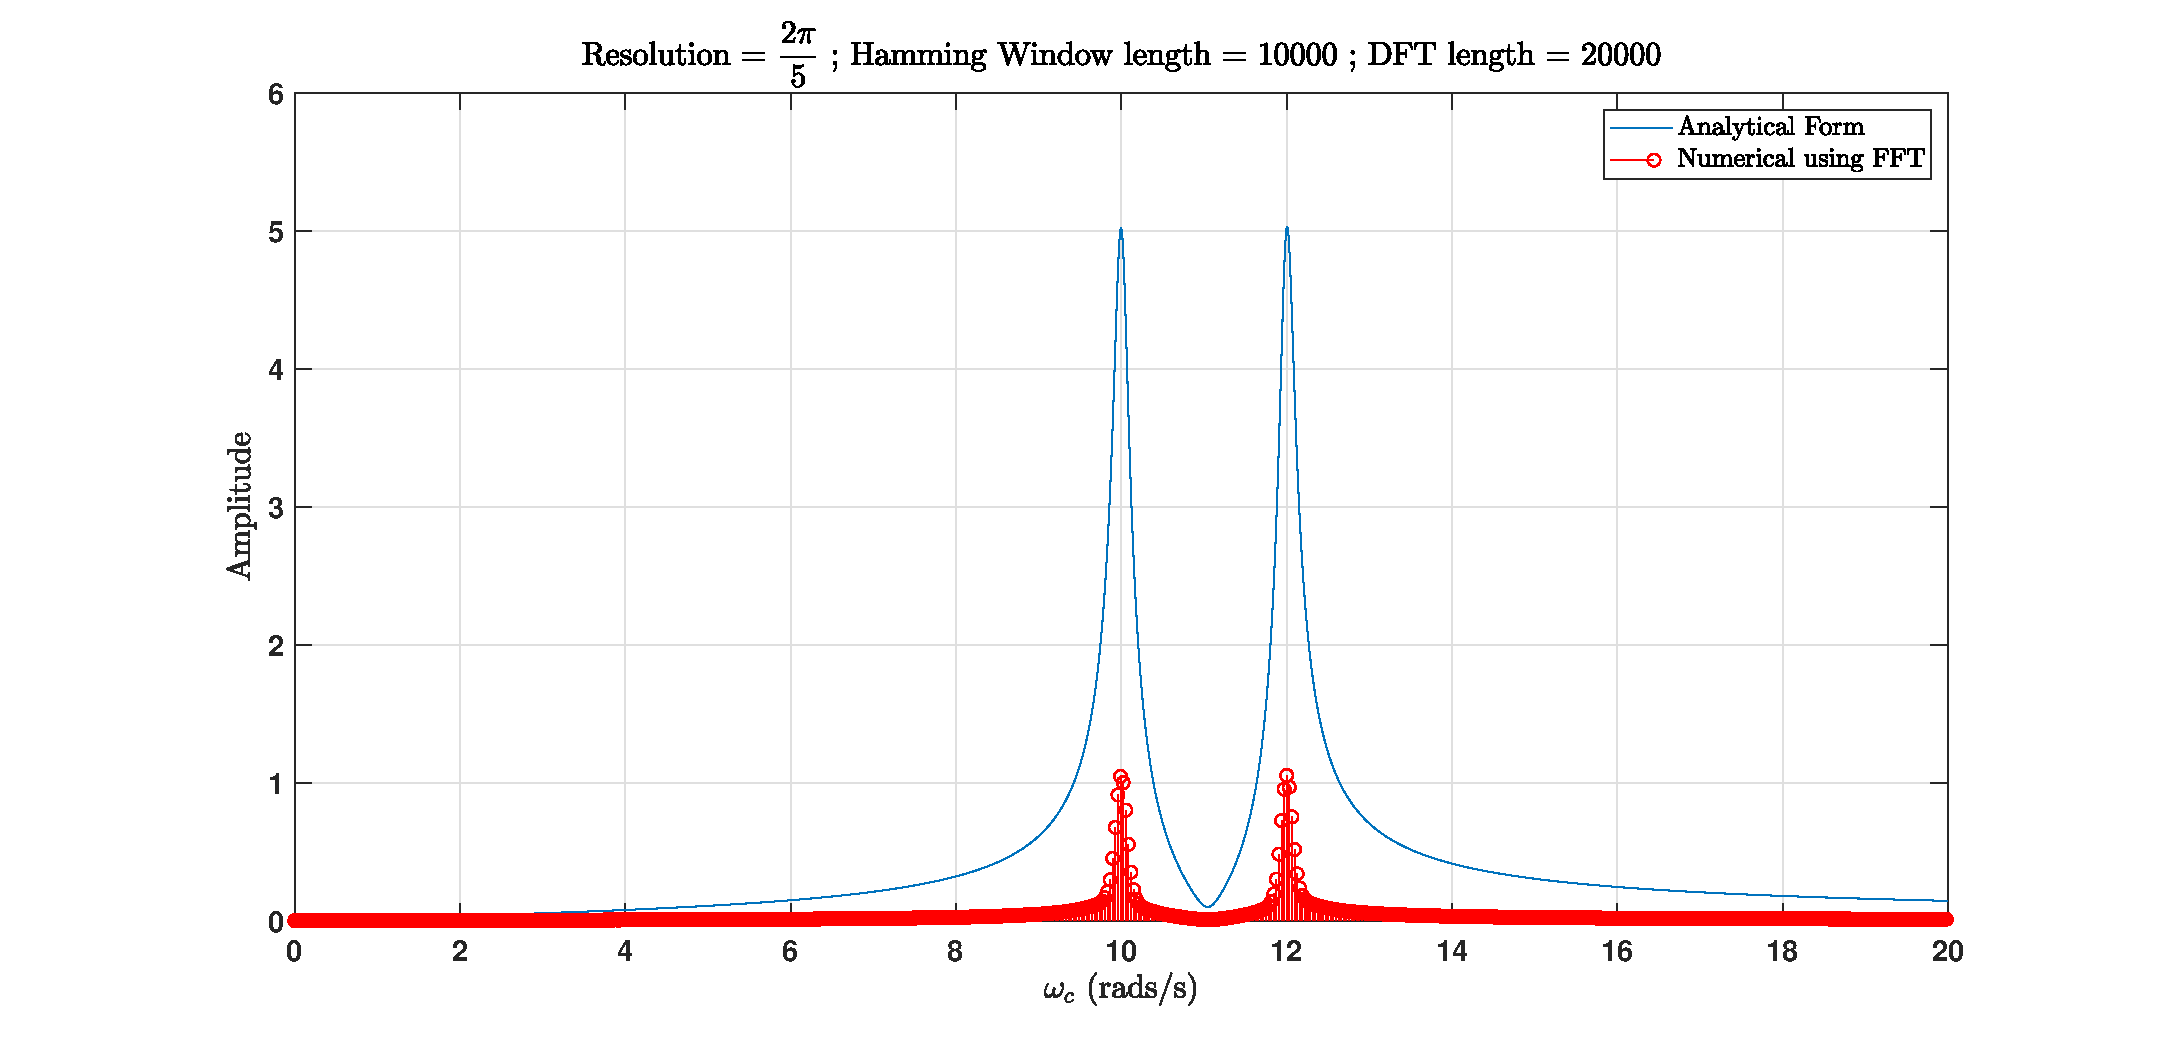
\includegraphics[scale=0.26]{Figures/DFT/spectrum_hamming_window_length_10_pow_4.eps}
\label{fig:DFT:spectrum_hamming_window_length_10_pow_4}
\end{figure}

\item DFT amplitude values are very distorted

\item Hamming is attenuating signal energy when we are windowing 

\begin{figure}[h]
\centering
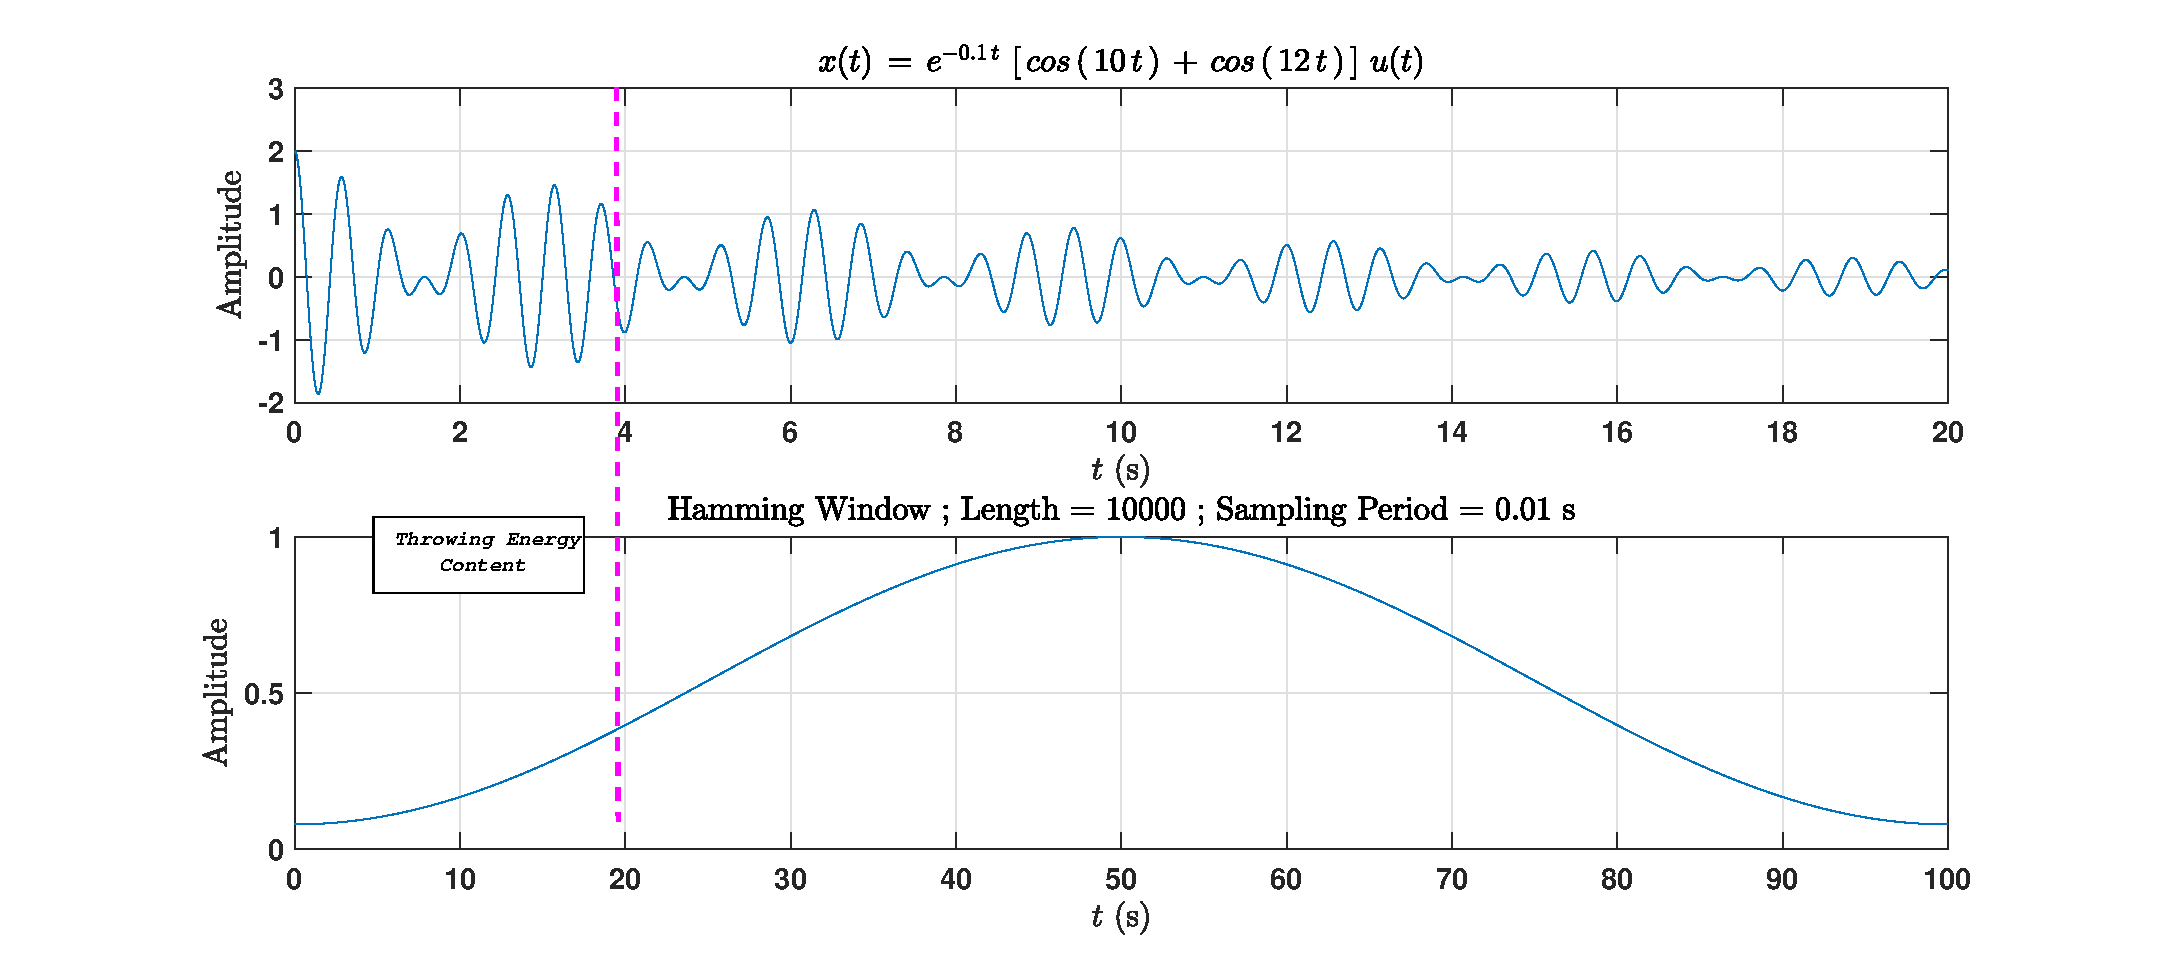
\includegraphics[scale=0.30]{Figures/DFT/hamm_signal_plot_time_domain_2.eps}
\label{fig:DFT:hamm_signal_plot_time_domain_2}
\end{figure}	
	

\end{itemize}


%***************************************
%***************************************
%***************************************